\documentclass[11pt, a4paper]{article}

\usepackage[utf8]{inputenc}
\usepackage{fullpage}
\usepackage{graphicx}
\graphicspath{ {images/} }
\usepackage{listings}
\usepackage[noend]{algpseudocode}
\renewcommand\algorithmicthen{}
\renewcommand\algorithmicdo{}
\usepackage{mathtools}
\usepackage{amssymb}
\usepackage{eurosym} %Euro symbol
\usepackage[ngerman]{babel}
\usepackage{cancel} %Kürzen
\usepackage{pbox}
\usepackage{tikz}

\newcommand\braces[1]{\left(#1\right)}
\newcommand\brackets[1]{\left[#1\right]}
\renewcommand{\vec}[1]{\underline{#1}}
\newcommand{\mat}[1]{\underline{\underline{#1}}}
\newcommand{\abs}[1]{\left\lvert#1\right\rvert}
\newcommand{\norm}[1]{\left\lVert#1\right\rVert}
\newcommand\tr[1]{\mathrm{tr}\br{#1}}
\newcommand\average[1]{\left\langle#1\right\rangle}
\newcommand{\acos}[1]{\mathrm{acos}\braces{#1}}
\newcommand{\asin}[1]{\mathrm{asin}\braces{#1}}
\newcommand{\dx}[1][x]{\ \mathrm{d#1}}
\newcommand\expectedValue[1]{\mathbb{E}\braces{#1}}
\newcommand\variance[1]{\mathbb{V}\braces{#1}}
\newcommand\setequal{\overset{!}{=}}
\newcommand{\gerquote}[1]{\glqq#1\grqq}
\newcommand{\T}{\ensuremath{\mathcal{T}} }
\newcommand{\D}{\ensuremath{\mathcal{D}} }
\newcommand{\bul}{\ensuremath{\bullet}}
\newcommand{\drawAtX}[3]{\draw (#1 |- 0,#2) to (#1 |- 5,#3)}

%\tikzset{every picture/.style=very thick}

\title{Algorithmische Geometrie Projekt \\ Trapezzerlegung}
\author{Phil Yannick Schrör \and Christian Mielers}
\date{\today}

% Warum in Python?

% TODO: Degenerierten Datensatz testen

\begin{document}
\maketitle

\section{Einleitung}


Der für Aufgabenteil 1 entwickelte Algorithmus besteht im Wesentlichen aus drei unterschiedlichen Teilen. Der erste Teil umfasst die Erstellung der Trapezzerlegung. Sobald diese erstellt wurde, müssen im zweiten Teil den Trapezen der Trapezzerlegung die entsprechenden Facetten der originalen Unterteilung der Ebene zugeordnet werden. Anschließend werden im letzten Teil alle jene Punkte zusammengefasst, welche einer Facette angehören. Die Umsetzung der einzelnen Teile wird in den folgenden Kapiteln genauer untersucht.\\
Für den zweiten Aufgabenteil verwenden wir die für Aufgabenteil 1 programmierte Trapezzerlegung zur Ermittlung eines hindernisfreien Pfades eines Roboters durch die mit Hindernissen versehene Ebene. Dabei halten wir uns im Allgemeinen an die Vorgehensweise, welche im Buch \gerquote{Computational Geometry} von Mark de Berg, Otfried Cheong, Marc van Kreveld und Mark Overmars in Kapitel 13.2 vorgestellt wird. Es kommt also ein RoadMap-Graph zum Einsatz, der zwecks Pfadfindung mittels Breitensuche traversiert wird.\\
Da die Programmiersprache Python 3 eine Vielzahl von komfortablen Datenstrukturen und Klassen zur Verfügung stellt und außerdem eine gute Leserlichkeit bietet, haben wir uns dazu entschlossen, das Programm in ebendieser Sprache zu programmieren.

\section{Annahmen}

Wie in der Aufgabenstellung angegeben, gehen wir im Rahmen dieses Projektes davon aus, dass sich alle Eingabepunkte in allgemeiner Lage befinden, also ganzzahlige Koordinaten haben, und keine zwei Punkte sich dieselbe x-Koordinate teilen. Dieser Umstand gewährleistet unter anderem, dass alle Nachbarn der Trapeze stets eindeutig definiert sind.

Darüber hinausgehend erwartet unsere Trapezzerlegung, dass sich der Startpunkt $p$ einer Strecke stets links von ihrem Endpunkt $q$ befindet. Diese Konvention führt zu einer nicht zu vernachlässigenden Verringerung benötigter Fallunterscheidungen und wird beim Einlesen der Daten hergestellt.

Um die Trapezzerlegung zu konstruieren, ist es erforderlich, alle von einer Linie geschnittenen Trapeze zu finden. Dies bedarf besonderer Behandlung, wenn zwei Strecken den selben Startpunkt haben. Um diesen herum liegen dann schon mindestens $2$ Trapeze, wie in Abbildung \ref{fig:intersected-trapezoids} dargestellt ist. Natürlich soll als erstes geschnittenes Trapez das rechte, 'echt' geschnittene gefunden werden. Hierfür könnte man sich entscheiden, bei Gleichheit der $x$-coordinaten rechts weiterzusuchen. Problematisch ist aber die Entscheidung, ob man im oberen oder unteren rechten Trapez suchen muss. Man könnte dies über die Winkel der ausgehenden Strecken eines Punktes lösen, die sich jeder Punkt dann merken müsste. Einfacher wird dies aber, wenn man ein minimales Verhältnis vom Abstand der Punkte der Zerlegung untereinander zur Länge der Strecken annimmt. Dann kann man einfach nach einem Punkt suchen, der auf der Strecke minimal hinter dem Startpunkt liegt, was in der Abbildung \ref{fig:intersected-trapezoids} durch ein Kreuz angedeutet ist. Unsere Entscheidung ist auf diese vereinfachte Variante gefallen.
\begin{figure}[h!]
	\centering
	\begin{tikzpicture}[scale=0.6]
		\begin{scope}[thick]
			\node (n1) at (2,6) {\bul};
			\node (n2) at (4,2) {\bul};
			\node (n3) at (5,4) {\bul};
			\node (n4) at (6,7) {\bul};
			\node (n5) at (8,2.5) {\bul};
			\node (n6) at (9,5) {\bul};
			\node (2eps) at (2.3,5.8) {$\times$};
		
			\draw (0,0) to (11,0) to (11,8) to (0,8) to (0,0);
			\draw (n1) to (n4);
			\draw (n4) to (n6);
			\draw (n2) to (n5);
			\draw[gray] (n1) to (n3);
		\end{scope}
		\begin{scope}[dashed,thick]
			\drawAtX{n1}{0}{8};
			\drawAtX{n2}{0}{6.5};
			\drawAtX{n4}{2.3}{8};
			\drawAtX{n5}{0}{5.6};
			\drawAtX{n6}{0}{8};
		\end{scope}
	\end{tikzpicture}
	\caption{Illustration zum Auffinden geschnittener Trapeze}
	\label{fig:intersected-trapezoids}
\end{figure}

\section{Objekte und Datenstrukturen}

Im Folgenden wird aufgeführt, welche Datenstrukturen zur Realisierung der Trapezzerlegung entwickelt wurden.

\subsection{Geometrische Objekte}

Wir haben uns dazu entschlossen, die geometrischen Objekte als Klassen zu implementieren, da auf diese Weise die Methoden, die im Algorithmus immer wieder Verwendung finden, komfortabel zur Verfügung gestellt werden können. Da diese Methoden auf einem Objekt aufgerufen werden, erspart dies auch die Übergabe einiger Parameter.\\
Die Klasse $\texttt{Point}$ speichert für einen Punkt seine $x$- und seine $y$-Koordinate. Weiterhin stellt sie Methoden zur Verfügung, welche überprüfen, ob ein übergebener Punkt links bzw. rechts vom betrachteten Punkt liegt. Außerdem existiert die Methode \texttt{is\_above(self, line)}, die überprüft, ob der Punkt überhalb der übergegebenen Strecke liegt.\\
Zur Repräsentation von Strecken dient die Klasse \texttt{Line}, welche sowohl einen Start- als auch einen Endpunkt speichert. Die Methode 
\texttt{eval(self, x\_coord)} ermittelt für die übergebene $x$-Koordinate die zugehörige $y$-Koordinate auf der durch die Strecke induzierten Linie.\\
Die Klasse \texttt{Trapezoid} speichert zum einen die Strecken, die es nach oben und unten begrenzen, und zum anderen die Punkte, welche die Lage der linken bzw. der rechten Kante des Trapezes bestimmen. Weiterhin werden für jedes Trapez seine Nachbarn gespeichert.
\begin{figure}[h!]
	\centering
	\begin{tikzpicture}[scale=0.8]
		\begin{scope}[very thick]
			\node (1) at (0,0) {\bul};
			\node (2) at (2,1.3) {\bul};
			\node (3) at (5,-0.1) {\bul};
			\node (0) at (-2,-0.2) {\bul};
		
			\draw[-,blue] (-3,1.87) to (6,2.9);
			\draw[-,blue] (-3,-1.43) to (6,-2);
			\draw[-,blue] (0) to (1);
			\draw[-,blue] (2) to (3);
			\draw[-] (0,-1.6) to (0,2.2);
			\draw[-] (2,-1.7) to (2,2.5);
			\draw[-] (5,-1.9) to (5,2.8);
			\draw[-] (-2,-1.45) to (-2,2);
		
			\node (A) at (1,0.5) {$A$};
			\node (B) at (3.5,1.6) {$B$};
			\node (C) at (3.5,-0.5) {$C$};
			\node (D) at (-1,-0.7) {$D$};
			\node (E) at (-1,1) {$E$};
		\end{scope}
	\end{tikzpicture}
	\caption{Ein Trapez mit vier Nachbarn}
	\label{fig:neighbors}
\end{figure}
In Abbildung \ref{fig:neighbors} ist ein Trapez $A$ gezeigt, welches vier Nachbarn hat. Wir haben uns dazu entschlossen, die Nachbarn entsprechend der Himmelsrichtungen zu bezeichnen, die sich durch den linken bzw. rechten Endpunkt ergeben. Somit ist $B$ der nordöstliche , C der südöstliche, D der südwestliche und E der nordwestliche Nachbar von $A$.

\subsection{Trapezzerlegung und Suchstruktur}

Als Datenstruktur für die Trapezzerlegung \T haben wir die Python-Klasse \texttt{set} verwendet, da diese zahlreiche Methoden für mathematische Mengen zur Verfügung stellt. Diese Methoden erreichen größenordnungsmäßig das Optimum (Laufzeit erwartet in der Größe der Mengen, Abfrage ob ein Element der Menge ist erwartet $\mathcal{O}(1)$). \T stellt zusätzlich eine Methode bereit, um alle von einer Linie geschnittenen Trapeze zu finden.
Für die Suchstruktur \D haben wir die neue Klasse \texttt{Tree} entworfen. Ein Objekt dieser Klasse hat zum einen ein Attribut, welches den Inhalt des Knotens (eine Strecke, einen Punkt oder eine Linie) speichert. Zum anderen speichert es einen Links- und einen Rechtsverweis auf sein linkes bzw. rechtes Kind. Das umschließende Trapez für einen Anfragepunkt $\rho$ liefert die Methode \texttt{find(self, point)}. Diese steigt den Baum hinab und prüft bei Punkten, ob $\rho$ links oder rechts davon liegt, bei Strecken ob $\rho$ darüber oder darunter liegt. Gemäß des Ergebnisses wird mit dem linken oder rechten Kind fortgefahren. Wird ein Blattknoten und damit ein Trapez erreicht, wird dieses als Antwort zurückgeliefert.

\section{Konstruktionsalgorithmus}

Zu Beginn der Konstruktion der Trapezzerlegung wird zunächst eine Bounding Box erzeugt und sowohl in \T als auch in \D eingefügt. Anschließend werden zwecks Randomisierung die Eingabestrecken in zufällige Reihenfolge gebracht. Daraufhin wird mit der Hauptschleife begonnen, in der pro Iteration eine Strecke zur Trapezzerlegung hinzugefügt wird.\\
Innerhalb der Schleife wird zunächst ermittelt, welche der bereits in die Trapezzerlegung eingefügten Trapeze von der einzufügenden Strecke geschnitten werden. Handelt es sich dabei um bloß ein Trapez, ist eine andere Behandlung erforderlich als wenn es sich um mehrere Trapeze handelt. Abbildung \ref{fig:one_trap_inside} zeigt den Fall, dass die neu eingefügt Strecke $\overline{pq}$ innerhalb exakt eines Trapezes liegt.
\begin{figure}[h!]
	\centering
	\begin{tikzpicture}[scale=0.8]
		\begin{scope}[thick]
			\node (1) at (-1,1.3) {\bul};
			\node (2) at (9,-1.95) {\bul};
	
			\draw[-] (-3,1) to (10,3);
			\draw[-] (-3,-1) to (10,-2);
			\draw[-] (1) to (-1,-1.1);
			\draw[-] ( 2) to (9,2.79);
		
			\node (3) at (1,0) {\bul};
			\node (4) at (7,0.5) {\bul};
			\draw[-] (3) to (4);
			\draw[-] (1,-1.3) to (1,1.57);
			\draw[-] (7,-1.8) to (7,2.5);
		
			\node (A) at (0,0) {$A$};
			\node (B) at (4,1.2) {$B$};
			\node (C) at (4,-0.7) {$C$};
			\node (D) at (8,0.5) {$D$};
			\node (p) at (.7,-0.2) {$p$};
			\node (q) at (7.3,0.4) {$q$};
		\end{scope}
	\end{tikzpicture}
	\caption{Die neue Strecke liegt innerhalb eines Trapezes.}
	\label{fig:one_trap_inside}
\end{figure}\\
Innerhalb dieses Falles gibt es neben dem dargestellten Fall noch drei weitere Fälle. Der Punkt $p$ könnte auf der linken Grenze von Trapez $A$ liegen, Punkt $q$ könnte auf der rechten Grenze von Trapez $D$ liegen und es könnte passieren, dass beide Fälle eintreten. Jeder dieser Fälle benötigt eine eigene Behandlung, da entweder Trapez $A$ nicht erzeugt werden muss, Trapez $D$ nicht erzeugt werden muss oder beide Trapeze nicht erzeugt werden müssen.\\
Liegt die einzufügende Strecke nur innerhalb eines Trapezes, gestaltet sich die Bestimmung der Nachbarn relativ einfach. Dies sei exemplarisch am in Abbildung \ref{fig:one_trap_inside} dargestellten Fall gezeigt. Hier müssen die westlichen Nachbarn des ursprünglichen Trapezes Trapez $A$ zugeordnet werden. Dies erfolgt analog mit den östlichen Nachbarn von Trapez $D$. Ferner erhalten $A$ und $D$ als östliche bzw. westliche Nachbarn die Trapeze $B$ (nördlich) und $C$ (südlich). Darüber hinaus müssen entsprechende Rückverweise von den Nachbarn des ursprünglichen Trapezes auf die neu erstellen Trapeze gesetzt werden.\\
Tritt der Fall auf, dass die neu eingefügte Strecke mehrere Trapeze $\Delta_1, \ldots, \Delta_n$ schneidet, gestaltet sich die Erstellung der neu einzufügenden Trapeze etwas schwieriger. Dazu betrachten wir das in Abbildung \ref{fig:multiple_traps} dargestellte Szenario. Anders als in Abbildung \ref{fig:one_trap_inside} wurden die neu einzufügenden Trapeze noch nicht in die Abbildung integriert.
\begin{figure}[h!]
	\centering
	\begin{tikzpicture}[scale=0.8]
		\begin{scope}[thick]
			\node (1) at (0,0) {\bul};
			\node (2) at (4,-2) {\bul};
			\node (3) at (5,1) {\bul};
			\node (4) at (9,2) {\bul};
			\node (5) at (12,-1) {\bul};
			\node (6) at (16,0) {};
		
			\draw[-] (1) to (6,2);
			\draw[-] (1) to (2);
			\draw[-] (3) to (5,1.6);
			\draw[-] (2) to (5);
			\draw[-] (3) to (4);
			\draw[-] (4) to (6);
		
			\draw[-] (2) to (4,1.3);
			\draw[-] (3) to (5,-1.8);
			\draw[-] (4) to (9,-1.35);
			\draw[-] (5) to (12,1.1);
		
			\node (7) at (2.7,0) {\bul};
			\node (8) at (10.6,0.5) {\bul};
			\draw[-,thick] (7) to (8);
			\node (p) at (2.4,-0.2) {$p$};
			\node (q) at (10.9,0.4) {$q$};
		
			\node (D1) at (1.7,-0.1) {$\Delta_1$};
			\node (D2) at (4.5,-0.6) {$\Delta_2$};
			\node (D3) at (7,-0.5) {$\Delta_3$};
			\node (D4) at (10.5,-0.2) {$\Delta_4$};
		\end{scope}
	\end{tikzpicture}
	\caption{Die neue Strecke liegt innerhalb mehrerer Trapeze}
	\label{fig:multiple_traps}
\end{figure}\\
Zunächst muss nun ein Trapez $A$ links vom Punkt $p$ erstellt werden. Anschließend werden überhalb und unterhalb der Strecke Trapeze erzeugt und gegebenenfalls erweitert. Zum Abschluss muss ein weiteres Trapez $G$ rechts vom Punkt $q$ erzeugt werden. Dies führt zu der in Abbildung \ref{fig:multiple_traps_2} dargestellten Situation.
\begin{figure}[h!]
	\centering
	\begin{tikzpicture}[scale=0.8]
		\node (1) at (0,0) {\bul};
		\node (2) at (4,-2) {\bul};
		\node (3) at (5,1) {\bul};
		\node (4) at (9,2) {\bul};
		\node (5) at (12,-1) {\bul};
		\node (6) at (16,0) {};
		
		\draw[-,thick] (1) to (6,2);
		\draw[-,thick] (1) to (2);
		\draw[-,thick] (3) to (5,1.6);
		\draw[-,thick] (2) to (5);
		\draw[-,thick] (3) to (4);
		\draw[-,thick] (4) to (6);
		
		\draw[-,thick] (2) to (4,0.05);
		\draw[-,thick] (3) to (5,0.18);
		\draw[-,thick] (4) to (9,0.38);
		\draw[-,thick] (5) to (12,1.1);
		
		\node (7) at (2.7,0) {\bul};
		\node (8) at (10.6,0.5) {\bul};
		\draw[-,thick] (7) to (8);
		\node (p) at (2.4,-0.2) {$p$};
		\node (q) at (10.9,0.4) {$q$};
		
		\draw[-] (2.7,-1.3) to (2.7,0.9);
		\draw[-] (10.6,1.5) to (10.6,-1.1);
		
		\node (A) at (1.5,-0.1) {$A$};
		\node (B) at (3.8,0.7) {$B$};
		\node (C) at (7,0.9) {$C$};
		\node (D) at (9.8,1.1) {$D$};
		\node (E) at (3.5,-0.7) {$E$};
		\node (F) at (7,-0.7) {$F$};
		\node (G) at (11.3,-0.2) {$G$};
	\end{tikzpicture}
	\caption{Die neue Strecke liegt innerhalb mehrerer Trapeze}
	\label{fig:multiple_traps_2}
\end{figure}\\
In unserem Algorithmus wird zunächst Trapez $A$ erstellt. Dessen westliche Nachbarn werden auf die Nachbarn von $\Delta_1$ gesetzt. Entsprechende Rückverweise werden ebenfalls gesetzt.
Anschließend beginnen wir mit einer Schleife, welche über die $\Delta_i$ Trapeze iteriert. Da die Behandlung oberhalb und unterhalb der Strecke analog erfolgt, wird im Folgenden nur die Behandlung der Trapeze oberhalb der Strecke dargelegt. Zu Beginn erzeugen wir ein neues Trapez $\Delta_u$, welches auf den verbleibenden Teil von $\Delta_1$ rechts von $p$ und oberhalb von der Strecke gesetzt wird. Dieses Trapez erhält Trapez $A$ als nordwestlichen Nachbarn und als nordöstlichen Nachbarn den nordöstlichen Nachbarn von $\Delta_1$. Anschließend betrachten wir das Trapez $\Delta_2$ oberhalb der Strecke und stellen fest, dass die obere Kante des Trapezes die gleiche ist wie bei $\Delta_u$. Somit müssen wir unser bisheriges $\Delta_u$ um den betrachteten Ausschnitt von $\Delta_2$ erweitern. Auch an dieser Stelle muss der nordöstliche Nachbar verändert werden, er wird auf den nordöstlichen Nachbarn von $\Delta_2$ gesetzt. Nun betrachten wir Trapez $\Delta_3$ oberhalb der Strecke. Wir stellen fest, dass hier die oberen Begrenzungskanten ungleich sind. Somit lassen wir unser bisheriges $\Delta_u$ unverändert und erstellen ein neues Trapez $\Delta_u$, welches einen Südwestverweis auf das bisherige $\Delta_u$ und einen Nordwestverweis auf den nordwestlichen Nachbarn von Trapez $\Delta_3$ erhält. Auch hier müsste der nordöstliche Nachbar gesetzt werden, diesmal auf den jedoch nicht existierenden nordöstlichen Nachbarn von Trapez $\Delta_3$. Wie immer werden auch hier die enstprechenden Rückverweise gesetzt. Auf diese Weise verfahren wir weiter, bis wir beim letzten Trapez angelangt sind.
Dort muss sowohl das rechteste Trapez rechtsseitig von Punkt $q$ erstellt werden als auch ermittelt werden, wie mit dem Ausschnitt von $\Delta_n$ links von Punkt $q$ zu verfahren ist. Es kann zum einen der Fall eintreten, dass das Trapez links von $q$ oberhalb der Strecke die gleiche obere Kante wie das letzte $\Delta_u$ hat. In diesem Fall werden beide Trapeze verschmolzen. Andernfalls werden sowohl das letzte $\Delta_u$ als auch der betrachtete Teil von $\Delta_n$ \T hinzugefügt. Das Setzen der Nachbarn erfolgt analog zu der Behandlung auf der linken Seite bei $\Delta_1$.\\
Tritt der Fall ein, dass $p$ auf der linken Grenze von $\Delta_1$ liegt oder $q$ auf der rechten Grenze von $q$ muss dort das linkeste bzw. das rechteste Trapez nicht erzeugt werden. Hier ist also ebenfalls eine Fallunterscheidung notwendig.

\section{Facettenzuweisung}
Ziel des Projektes ist es, die Indizes der Punkte innerhalb einer Facette in eine Zeile der Ausgabedatei zu schreiben. Problematisch ist hierbei, dass als Eingabedaten nur die Strecken, die die Ebene unterteilen zur Verfügung stehen. Eine Zuordnung der jeweiligen Seiten der Strecken zu Facetten ist dagegen nicht gegeben. Somit muss die Zuordnung der erstellten Trapeze zu der passenden Facette noch berechnet werden. Hier ist die zentrale Beobachtung, dass zwei Trapeze in einer Facette liegen, wenn sie einander über Nachbarschaftsbeziehungen (evtl. mit Zwischentrapezen) erreichen können. Ein geeigneter Algorithmus ist also

\begin{algorithmic}[1]
\State Input: trapezoid t, face f
\Function{assign face}{t, f}
	\If {t has no face assigned}
		\State assign t to f
		\ForAll {neighbors of t}
			\State \Call{assign face}{n, f}
		\EndFor
	\EndIf
\EndFunction

\State Input: Decomposition T
\Function{assign faces}{T}
	\ForAll {$t \in T$}
		\State f $\gets$ new Face
		\State \Call{assign face}{t, f}
	\EndFor
\EndFunction
\end{algorithmic}

wobei jede Facette von einem Starttrapez aus über die Nachbarschaftsverweise traversiert wird, wie in Abbildung \ref{fig:face-assignment} dargestellt ist. Startet man in dem mit $\times$ markierten Trapez, läuft man entlang der Nachbarschaftsverweise die komplette Facette ab.

\begin{figure}[h!]
	\centering
	\begin{tikzpicture}[scale=0.5]
		\begin{scope}[thick]
			\draw (-2,-4) to (11,-4) to (11,5) to (-2,5) to (-2,-4);
			
			\node (n1) at (0,0) {\bul};
			\node (n2) at (2,2) {\bul};
			\node (n3) at (6,3) {\bul};
			\node (n4) at (9,1) {\bul};
			\node (n5) at (4,-2) {\bul};
			\draw (n1) to (n2) to (n3) to (n4) to (n5) to (n1);
		\end{scope}
		
		\begin{scope}[dashed]
			\drawAtX{n1}{-4}{5};
			\drawAtX{n2}{-1}{5};
			\drawAtX{n3}{-0.8}{5};
			\drawAtX{n4}{-4}{5};
			\drawAtX{n5}{-4}{2.6};
		\end{scope}
		
		\node (X) at (3,1) {$\times$};
		\draw[->] (X) to (5,1.5) node[below]{$1$};
		\draw[->] (5.2,1.5) to (7,1) node[below]{2};
		\draw[->] (X) to (1.5,0.5) node[above]{3};
		
		\node[draw,rectangle] at (1.5,-0.1) {5};
		\node[draw,rectangle] at (3,0.0) {5};
		\node[draw,rectangle] at (7.8,0.9) {5};
		\node[draw,rectangle] at (5,0.1) {5};
		
		\node[draw,rectangle] at (-1,1) {4};
		\node[draw,rectangle] at (1,3) {4};
		\node[draw,rectangle] at (4,4) {4};
		\node[draw,rectangle] at (7.5,3.5) {4};
		\node[draw,rectangle] at (10,1) {4};
		\node[draw,rectangle] at (2,-2.5) {4};
		\node[draw,rectangle] at (7,-2) {4};
	\end{tikzpicture}
	\caption{Darstellung der Nachbarschaftstraversierung bei der Facettenzuweisung}
	\label{fig:face-assignment}
\end{figure}

In unserer Implementierung ist eine Facette eine inkrementierende Integer-Variable (die, anders als hier vereinfachend dargestellt, nur inkrementiert wird, wenn nötig), die dem Trapez-Objekt als Attribut hinzugefügt wird. Damit ist es in konstanter Zeit möglich, von dem Trapez auf die Facette zu schließen. Da die Zuweisung in jeder Facette nur einmal gestartet wird und jedes Trapez innerhalb einer Facette höchstens von $4$ Nachbarn 'betreten' wird, ist die Laufzeit der Zuweisung $\mathcal{O}(\abs{T})$ und damit $\mathcal{O}(m)$, wobei $m$ die Anzahl der Strecken ist.

\section{Punktgruppierung}
Um die Punkte in der selben Facette in eine Zeile schreiben zu können, müssen sie zunächst nach Facette gruppiert werden. Die Facetten, zu denen die $l$ Abfragepunkte gehören, können in erwartet $\mathcal{O}(l \log m)$ bestimmt werden, wobei $m$ die Anzahl der Strecken ist.

\begin{algorithmic}[1]
\State Input: Search structure D, query points Q
\State Output: $Q_1 \dots Q_F$ sets of points for each face
\Function{group points}{D, Q}
	\ForAll {$q \in Q$}
		\State $t \gets$ \Call {D.find\_trapezoid}{q}
		\State $f \gets$ face of $t$
		\State add $q$ to $Q_f$
	\EndFor
\EndFunction
\end{algorithmic}

Die einzelnen Gruppen werden in unserem Programm als Python \texttt{list} vorgehalten, die ein Anfügen eines Punktes in $\mathcal{O}(1)$ erlauben. Um ohne explizite Repräsentation der Facetten (es gibt kein Facetten-Objekt oder Ähnliches) von der Integer-Variable, die den Facettenindex angibt, zu der entsprechenden Liste zu gelangen, werden die Listen in einer Hashmap (Python-\texttt{dictionary}) mit Facettenindex gespeichert, so dass das Finden der gesuchten Liste in erwartet $\mathcal{O}(1)$ möglich ist.

\section{Performance}
Zum Testen der Performance wurden Testdatensätze generiert, die automatisch von einem weiteren Python3-Programm erstellt werden. Diese entsprechen der Form nach einem gescherten Lattenrost, exemplarisch dargestellt in Abbildung \ref{fig:generated_dataset}. Zusätzlich wird für jede Facette ein Abfragepunkt generiert, der an einem zufälligen Ort in der Facette liegt.

\begin{figure}[h!]
	\centering
	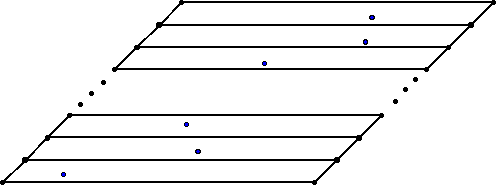
\includegraphics[width=0.75\textwidth]{generated_dataset}
	\caption{Darstellung der generierten Testdaten, Abfragepunkte in Blau}
	\label{fig:generated_dataset}
\end{figure}

Auf derartigen Datensätzen unterschiedlicher Größe wurde die Laufzeit der 3 Hauptbestandteile des Algorithmus, der Trapezzerlegung, der Facettenzuweisung und der Punktgruppierung, gemessen. Die Zeiten sind in Tabelle \ref{tab:performance_table} eingetragen und in Abbildung \ref{fig:performance_plot} graphisch dargestellt. Bei der Abbildung sei besonders auf die logarithmische Skala auf beiden Achsen hingewiesen. Die Daten wurden mit einem \texttt{i5-2430M} Prozessor unter \texttt{Python 3.4.0} erhoben

\begin{table}[h!]
	\centering
	\begin{tabular}{|r|r|c|c|c|}
		\hline
		m & l & Zerlegung $(s)$ & Facettenzuweisung $(s)$ & Punktgruppierung $(s)$ \\
		\hline
		7 & 2 & 0.0007 & 0.0001 & 0.0001 \\
		34 & 11 & 0.0033 & 0.0002 & 0.0003 \\
		304 & 101 & 0.0424 & 0.0013 & 0.0037 \\
		3004 & 1001 & 0.3959 & 0.0101 & 0.0440 \\
		30004 & 10001 & 5.2805 & 0.1220 & 1.2981 \\
		\hline
	\end{tabular}
	\caption{Laufzeiten der Zerlegung, der Facettenzuweisung und der Punktgruppierung für verschiedene Anzahlen von Zerlegungskanten $m$ und Abfragepunkten $l$}
	\label{tab:performance_table}
\end{table}

\begin{figure}[h!]
	\centering
	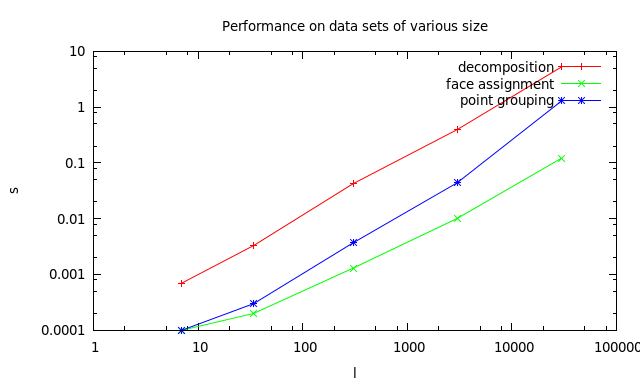
\includegraphics[width=\textwidth]{performance}
	\caption{Plot der Laufzeiten der Zerlegung, der Facettenzuweisung und der Punktgruppierung über die Anzahl der Zerlegungskanten $m$ in Sekunden}
	\label{fig:performance_plot}
\end{figure}

Hierbei lässt sich feststellen, dass alle 3 Werte näherungsweise linear wachsen. Ein leichter superlinearer Trend lässt sich allerdings visuell bei der Punktgruppierung erahnen. Die Trapezzerlegung ist mit einigem Abstand die langwierigste Operation, wobei hierbei ohnehin der größte konstante Faktor zu erwarten wäre. Da die Lokalisierung eines Punktes in erwartet $\mathcal{O}(\log n)$ läuft, ist die erwartete Laufzeit für das Lokalisieren in $\mathcal{O}(n \log n)$. Dies entspricht auch der insgesamt erwarteten Laufzeit für den Gruppierungsteil, da das Gruppieren der lokalisierten Punkte über das Einfügen in ein \texttt{Python-Dictionary} in amortisiert konstanter Zeit realisiert ist.

\appendix
\section{Programmnutzung}
Bei den Programmen zur Trapezzerlegung und Pfadsuche handelt es sich um Python3-Programme. Daher muss auf der Zielplattform eine Python3-Runtime installiert sein, das ältere Python2 wird nicht unterstützt. Darüber hinaus weisen die Programme keine externen Abhängigkeiten (etwa zu Drittbibliotheken) auf.

\paragraph{Trapezzerlegung} Die Trapezzerlegung wird in der Datei \texttt{trapezoid\_decomposition.py} realisiert. Die Syntax zum Programmaufruf lautet

\begin{quotation}
	\texttt{python3 trapezoid\_decomposition.py [-h] [-i] [-d] [-l] in\_file out\_file}
\end{quotation}

\begin{tabular}{|l|c|l|}
	\hline
	Parameter & erforderlich & Bedeutung \\
	\hline
	in\_file & * & \pbox{10cm}{Der Pfad zur Eingabedatei, in der die Punkte, Strecken und Abfragepunkte gespeichert sind} \\
	out\_file & * & Der Pfad zur Datei, in die die Ausgabe geschrieben wird \\
	h & & Hilfe zum Programmaufruf anzeigen \\
	i & & Die Eingabedaten (\textbf{i}nput) visualisieren \\
	d & & Die Zerlegung (\textbf{d}ecomposition) visualisieren \\
	l & & Lokalisierungsergebnisse (\textbf{l}ocalization) visualisieren \\
	\hline
\end{tabular}

Die Visualisierungsoptionen können alle im selben Aufruf genutzt werden.

\paragraph{Pfadsuche} Die Pfadsuche mittels Trapezzerlegung wird in der Datei \texttt{path\_finding.py} realisiert. Die Syntax zum Programmaufruf lautet

\begin{quotation}
	\texttt{python3 path\_finding.py [-h] [-d] [-r] [-p] in\_file out\_file}
\end{quotation}

\begin{tabular}{|l|c|l|}
	\hline
	Parameter & erforderlich & Bedeutung \\
	\hline
	in\_file & * & \pbox{10cm}{Der Pfad zur Eingabedatei, in der die Hindernisse und Start- sowie Endpunkte der zu findenden Pfade gespeichert sind} \\
	out\_file & * & \pbox{10cm}{Der Pfad zur Datei, in die die gefundenen Pfade geschrieben werden} \\
	h & & Hilfe zum Programmaufruf anzeigen \\
	d & & \pbox{10cm}{Die Trapezzerlegung (\textbf{d}ecomposition) der Eingabedaten visualisieren, nachdem die Hindernis-Trapeze entfernt wurden} \\
	r & & Die \textbf{R}oad-map visualisieren \\
	p & & Die gefundenen Pfade (\textbf{p}aths) visualisieren \\
	\hline
\end{tabular}

Die Visualisierungsoptionen können alle im selben Aufruf genutzt werden.

\end{document}










